%TODO: What other methods exist? What are the differences? What are the difficulties with other methods? How does it compare to a baseline method?

%\href{https://www.math.leidenuniv.nl/scripties/BSC-Obbens.pdf}{Interisting stuff} \cite{obbens2014inference}

\subsection{Bayesian networks} \label{sec:bayes}
% 2 page

As the Markov network, the Bayesian network is also a method for representing probabilistic models with a graph. Since the roots of Bayesian networks lie in path analysis by Right in 1921 \cite{wright1921correlation} and 1934 \cite{wright1934method}, this method of representation is slightly older than the Markov networks, which was firstly introduced by Barlett in 1935 \cite{bartlett1935contingency}.

The main difference between the Bayesian and the Markov network is that the first one has directed edges whereas the second has undirected ones. Furthermore the Bayesian network is restricted to be acyclic. This means that the dependency between two random variables can never be mutual but only one-directional. Thus, the edge $(A, B)$ would indicate that $B$ depends on $A$ and that their is no path from $B$ to $A$, which means that $A$ is the cause and $B$ the effect in this particular relation.

In the contrary to Markov networks the Bayesian network is able to assign the parameters by using probabilities. Because of the condition, that the graph is an acyclic directed graph, the number of variables, on which a variable $X$ depends, is equal to the number of its incoming edges. Using conditional probability distributions (CPD) a probability is assigned to each assignment times the number of values of $X$. The sum of probabilities of a \textit{CPD} is equal to one. When inferring on a Bayesian network the factor multiplication is similar to the Markov network: Multiply the probabilities of \textit{CPDs}, such that the assignments match up. Figure \ref{fig:bayes} shows a simple Bayesian network with four binary variables and their conditional probability distributions. As described above the summation over the product of \textit{CPDs} is calculated for inferring on the Bayesian network. Equation shows an example calculation for computing $P(D = d_T).$ The result of the example inference is, that $D$ is with a certainty of 64\% true.

\begin{equation}
P(D = d_T)=\sum_A{\sum_B{\sum_C{P(A)P(B|A)P(C)P(d_T|B,C)}}} = 0.64
\label{eq:bayes}
\end{equation}

\begin{figure}[htpb]
  \centering
  	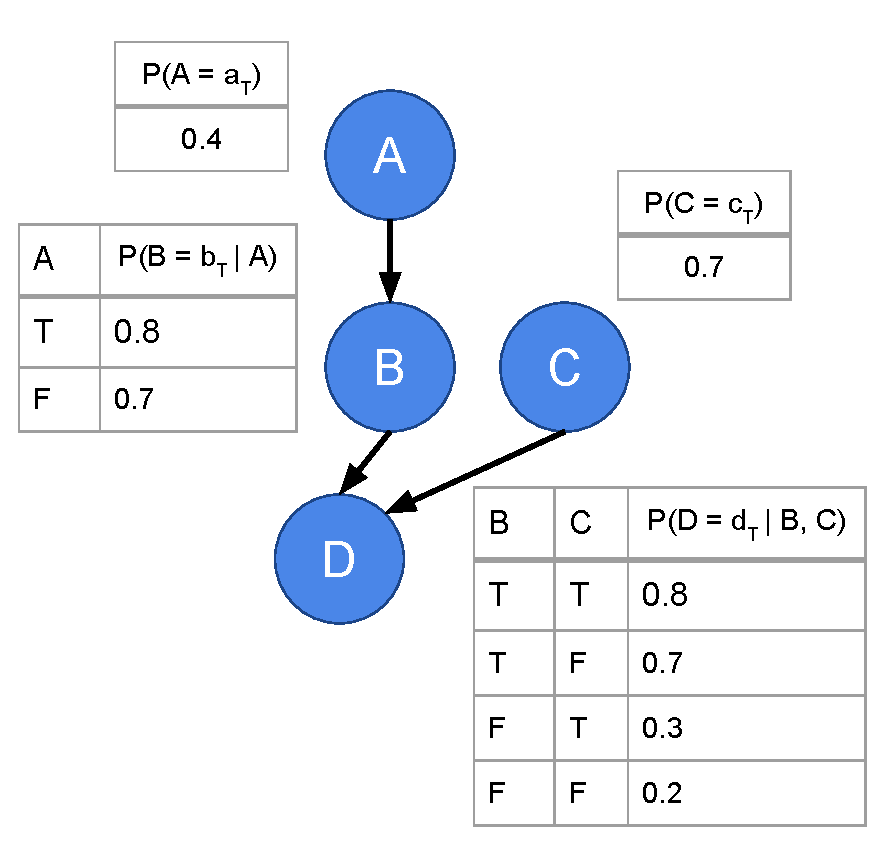
\includegraphics[scale=0.6]{img/bayes.pdf} 
  \caption{Examples of a Bayesian network including the conditional probability distributions}
  \label{fig:bayes}
\end{figure}

Since the affinities among assignments of random variables are expressed as probabilities, the adjustment of the parameters are not as flexible as in Markov networks.
% TODO: example, why is that?

In section \ref{sec:indep} the independences of a variable given a certain set of other variables was described as local Markov property using the Markov blanket for the Markov network. Also in Bayesian networks every node has a Markov blanket, for which holds that: Given the Markov blanket of a node, this node is independent from all variables unequal to the Markov blanket and the node itself. In Bayesian networks the Markov blanket includes the parents, the children and the other parents of the children. Using this property, the inference on those networks can be elevated dramatically in terms of computation time and space.

% TODO: Transformation of Bayesian network to Markov network and vise versa

%\subsection{Partially directed models}
% 1 page
% not sure of this
%- chapter 4.6


\subsection{Markov logic network} \label{sec:mln}
% 1.5 page

In 2006 Matthew Richardson and Pedro Domingos from the University of Washington in Seatle proposed to combine first-order logic with probabilistic graphical models and named it Markov logic network \cite{richardson2006markov}. This section describes what a Markov logic network is, how it extends the Markov network and discusses the benefits of this approach and what types of problems it solves.

% TODO: what is first-order logic, cite
In Markov logic network is build upon a first-order knowledge base, which is a set of sentences or formulas in first-order logic. The components of this sentences are constants as fixed objects of the domain, variables as a not fixed object of the domain, predicates, which present either relations between or attributes of objects, and finally functions as maps from tuples of object onto another object. A sentence is a logical combination of predicates and functions over constants and variables. Logical expressions can include negations, conjunctions, disjunctions, implications, equivalence and the universal and existential qualifier. For example if the domain consists of ${Anna, Bob, Carla}$ and there is a predicate $siblings(X,Y)$ the following first order logic sentence can be build:

\begin{equation}
siblings(Anna, Bob) \land siblings(Bob, Carla) \Rightarrow siblings(Anna, Carla)
\label{eq:logicexample}
\end{equation}

This can be generalized by using variables. Formula \ref{eq:logicexamplegen} states that if $a$ and $b$ and $b$ and $c$ are siblings then also $b$ and $c$ are siblings. This sentence does not consider half siblings.

\begin{equation}
\forall a\ \forall b\ \forall c\ siblings(a, b) \land siblings(b, c) \Rightarrow siblings(a, c)
\label{eq:logicexamplegen}
\end{equation}

In section \ref{sec:param} the parameterization of Markov networks using log-linear models, was described. Since logical knowledge bases include binary sentences, so that the sentence is either true or false, the goal of Markov logic networks is to soften those constraints by assigning weights to them. This represents, how likely a sentence is true or not. The set of pairs of formulas and their weights and the finite set of constants in the domain define the Markov network as a representation of the weighted knowledge base as follows. For each predicate which appears in the knowledge base a binary node is defined. Furthermore for each formula a feature, which has the same weight as the formula, is defined. Thus, the features are binary and referred to as indicator features, as described in the log-linear model in section \ref{sec:param}.

The following example is guided by the example provided by Richardson \cite{richardson2006markov} and shall illustrate, how to derive a Markov network from the knowledge base and the domain set of a Markov logic network. Let their be two formulas. The first one states, that a person will get a job if he studied. Secondly, two persons that are friends either studied both or neither of them did. Furthermore real number weights would be assigned to those both formulas. Hence, figure \ref{fig:mln} shows the regarding Markov network for the domain ${Anna,Bob}$.
Richardson provides the following example in his paper \cite{richardson2006markov}

\begin{figure}[htpb]
  \centering
  	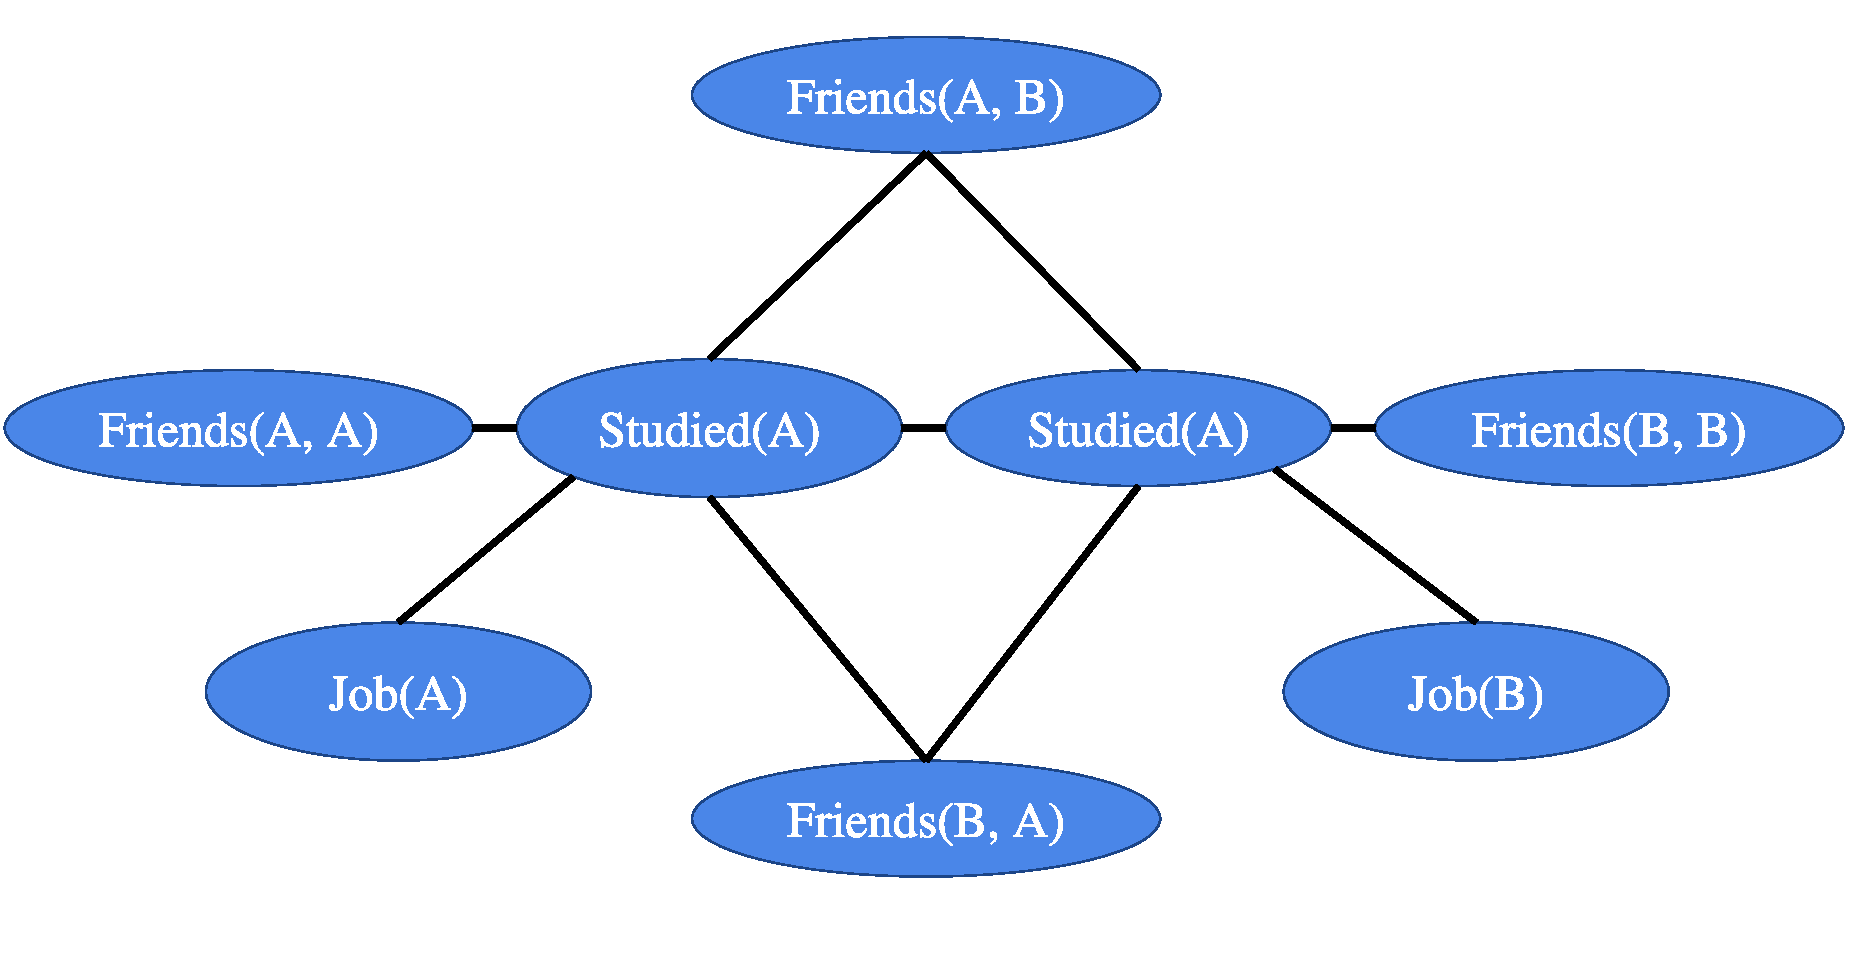
\includegraphics[scale=0.4]{img/mln.pdf} 
  \caption{Example Markov network derived from a knowledge base with the constants Anna(A) and Bob(B), guided by figure 1 in \cite{richardson2006markov}}
  \label{fig:mln}
\end{figure}

Thus, Markov logic networks extends the capabilities by utilizing the log-linear model representation of Markov networks to embed first-order logic. Hence, all algorithm, which can be applied on Markov networks can also be applied on Markov logic networks. For example inference can be done by querying the Markov network if a formula $F_1$ is likely to hold under the condition that a set of evidence predicates are true. Hence, the inference algorithms, like the variable elimination, described in section \ref{sec:infer} can be utilized to calculate such probability. When learning on a Markov logic network, the goal is to learn the weights of the formula, such that the probability distribution in the Markov logic network models the learned distribution. This can be applied in different areas like link prediction, social network modeling, object identification and various classifications \cite{richardson2006markov}. Cirn et al., for example, utilized the Markov logic network to classify topics in political manifestos in 2016 \cite{zirn2016classifying}.


